
\subsection{Введение}


\begin{to_def}
    \textit{Оптический волновод} -- диэлектрическая структура, по которой может распространяться электромагнитная энергия в видимой и инфракрасной областях спектра. 
\end{to_def}

Можно выделить ступенчатый и градиентный профиль волновода (рис. \ref{waveguide}).
\begin{figure}[ht]
    \centering
    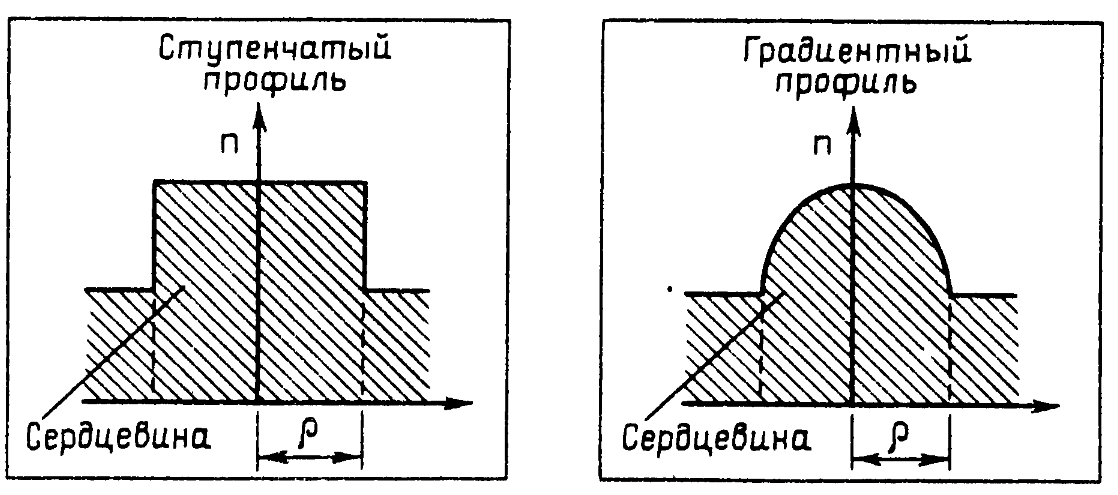
\includegraphics[height=0.17\textwidth]{figures/13_1.png}
    \hspace{5 mm} 
    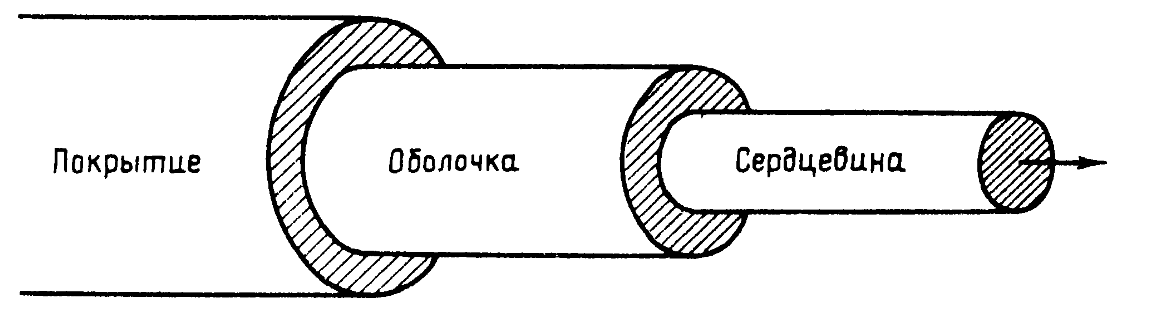
\includegraphics[height=0.12\textwidth]{figures/13_2.png}
    \caption{Профиль показателя преломления для типичных оптических волокон.}
    \label{waveguide}
\end{figure}
Обычно покрытие оказывается полностью изолировано от сердцевины, так что его влиянем можно пренебречь. 


\textbf{Многомодовые и одномодовые волноводы}. Оптические волноводы можно условно разделить на две группы -- \textit{многомодовые} (большая сердцевина) и \textit{одномодовые} (маленькая сердцевина). Для многомодовых световодов справедлво условие
\begin{equation*}
    \frac{2\pi \rho}{\lambda} \sqrt{\sub{n}{co}^2 - \sub{n}{cl}^2} \gg 1,
\end{equation*}
где $\rho$ -- характерный размер сердцевины, $\lambda$ -- длина волны света в свободном пространстве, $\sub{n}{co}$ -- максимальное значение показателя преломления сердцевины, а $\sub{n}{cl}$ -- показатель преломления оболочки. 
% см. часть I
%  часть II -- одномодовые

\textbf{Лучевой подход}. Показатель преломления обычно слабо меняется на масштабах $\lambda$ (по крайней мере для многомодовых), таким образом адекватно описывать происходящее в терминах лучей. 
В таком\footnote{
    Альтернативный подход к описанию распространения света в многомодовых волноводах -- коротковолновое приближение для ЭМ волн. 
}  случае \textit{пренебрегается всеми волновыми эффектами}. 
% см. гл. 6-9, локальные плоские волны


Важно, что в линиях связи большой протяженности случается уширение распространяющихся импульсов. В случе идеальных многомодовых волоконных световодов уширение вполне описывается геом-оптикой. 

